\section {LArTPC Detectors}


\begin{frame}
  \frametitle{LArTPC Experiments - ICARUS}

  The origin of LArTPC technology for Neutrinos: \href{http://cds.cern.ch/record/117852/files/CERN-EP-INT-77-8.pdf}{C. Rubbia, 1977} led to \textbf{ICARUS, the first, large-scale LArTPC}.

  \begin{columns}
    \begin{column}{0.5\textwidth}
      \begin{itemize}
      \item $2\times$ \SI{300}{\tonne} modules.
      \item Took data in the Gran Sasso tunnel, Italy from CERN
        neutrino beam.
      \item Moving to Fermilab as part of the \textbf{Short-Baseline
        Neutrino} Program.
      \end{itemize}
    \end{column}
    \begin{column}{0.5\textwidth}
      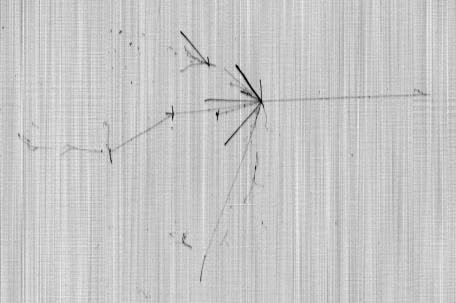
\includegraphics[width=0.8\textwidth]{icarus.png}
    \end{column}
  \end{columns}
\end{frame}

\begin{frame}
  \frametitle{LArTPC Experiments - MicroBooNE}

  \begin{center}
    Recently started taking $\nu$-data at Fermilab!    
  \end{center}

  \begin{columns}
    \begin{column}{0.5\textwidth}
      \begin{center}
        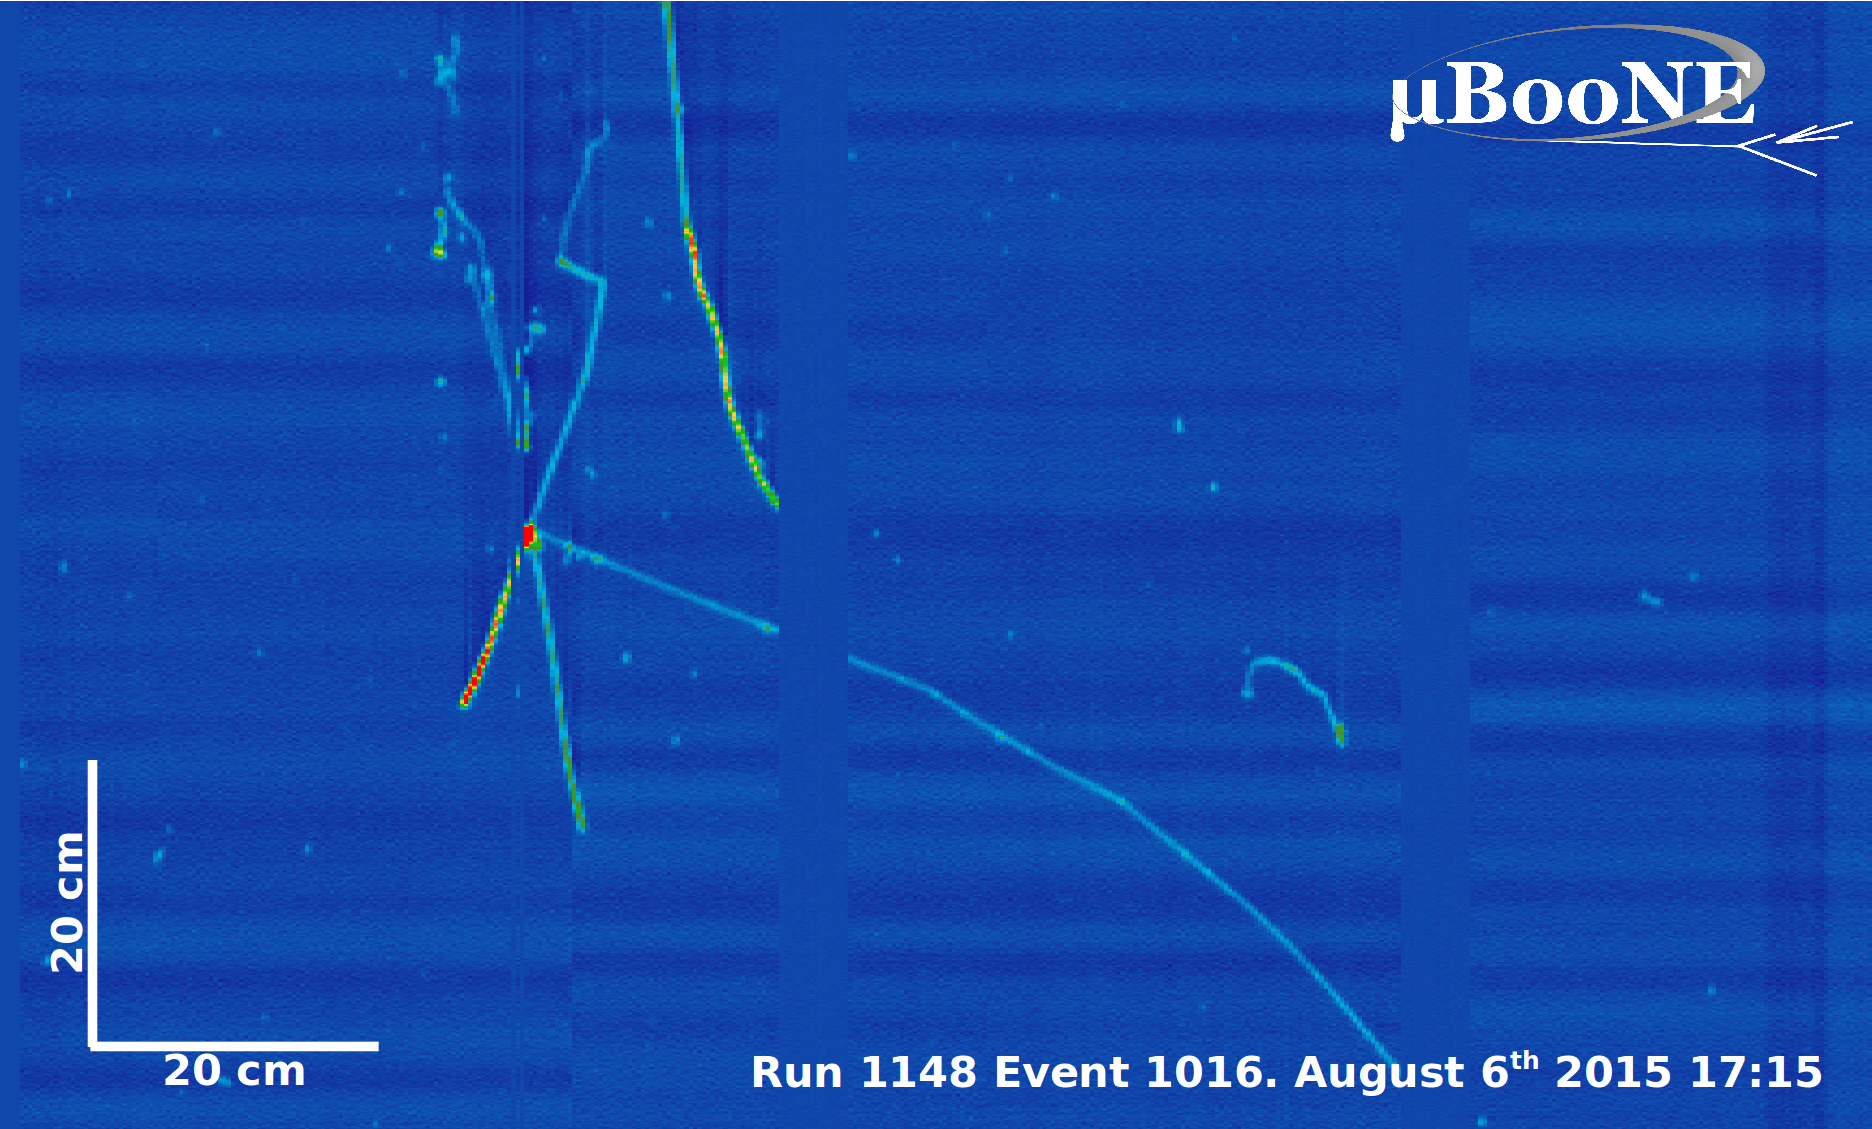
\includegraphics[width=0.9\textwidth]{run1148_ev1016.png}
      \end{center}

    \end{column}
    \begin{column}{0.5\textwidth}
      \begin{itemize}
      \item 85 ton fiducial mass.
      \item 8256 channels
      \item 3 mm wire pitch.
      \item Investigate:
        \begin{itemize}\footnotesize
        \item low energy excess puzzle
        \item sterile-$\nu$ search
        \item $\nu$-Ar cross sections
        \end{itemize}
      \end{itemize}
    \end{column}
  \end{columns}

  \vspace{3mm}

  \begin{center}
    MicroBooNE is the initial test bed for Wire Cell reconstruction.    
  \end{center}

\end{frame}

\begin{frame}[fragile]
  \frametitle{LArTPC Experiments - 
\includegraphics[height=7mm,trim=4cm 9.2cm 4cm 9.3cm,clip,valign=c]{DUNElogo_colorHORIZONTAL.pdf}}
  \begin{center}
    ``International \textbf{mega-science} project''

    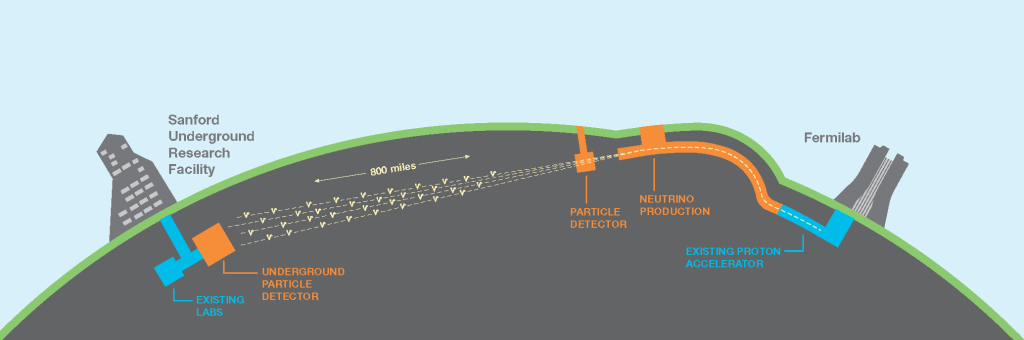
\includegraphics[height=25mm]{LBNF_Graphic_021715-1024x340.png}
  \end{center}


  Three stages of DUNE LArTPC detectors:
  \begin{enumerate}\footnotesize
  \item ``\textbf{35ton}'' prototype (at FNAL), just started operating, cosmic-$\mu$ exposure. 
  \item Full-scale ``\textbf{protoDUNE}'' (at CERN) 2017/2018 with $\pi, K, p$ beam tests.
  \item Full ``\textbf{DUNE}'' far detector underground in South Dakota $\sim$2025.
    \begin{itemize}
    \item At least \textbf{10 kt} of single-phase LAr, 3-plane, wire readout: \\
      5 mm wire pitch, \textbf{375K channels}.

    \item Total of \textbf{40 kt fiducial mass} in \textbf{4 separate cryostats}, \\
      \footnotesize{different technologies possible for each module.}

    \end{itemize}
  \end{enumerate}

\end{frame}

\begin{frame}
  \frametitle{LArTPC with Wire Readout - Basics Principles}

  \begin{itemize}
  \item Charged particles produce tracks of ionized LAr
  \item Electrons drift in an applied electric field 
    \begin{itemize} \footnotesize
    \item Eg: E = \SI{500}{\volt/\cm}, $v_{\mbox{drift}}=$ \SI{1.6}{\milli\meter/\micro\second}
    \end{itemize}
  \item Charge drifts past 3 parallel wire planes (\num{3}-\SI{5}{\milli\meter} pitch)
    \begin{itemize}
    \item 2 induction planes with bipolar signals.
    \item 1 collection plane with monopolar signals.
    \end{itemize}
  \item Digitize wire signal waveforms (\SI{2}{\mega\hertz}, 12 bits)
  \item Deconvolve detector response and apply noise filter.
  \item Optical system gives prompt $T_0$ from scintillation light.
  \end{itemize}

  \begin{itemize}
  \item [$\rightarrow$] Gives \textbf{three independent measures} of
    each element of drifting charge as \textbf{three, 2D views} (in \textbf{wire
    vs time}) which \textbf{multiplex the two transverse dimensions}.
  \end{itemize}

  \vfill

  \flushright\footnotesize{(animation by Bo Yu $\rightarrow$)}

\end{frame}

\begin{frame}[fragile]
  \begin{center}
      \multiinclude[<+->][format=png, graphics={trim=0cm 1.6cm 0cm 2cm, clip,height=0.9\textheight}]{signal}
  \end{center}
\end{frame}

\begin{frame}
  \frametitle{LArTPC Data}
  
  \vspace{-10mm}

  \begin{columns}
    \begin{column}{0.8\textwidth}
      LArTPC can produce \textbf{huge quantities} of \textbf{high-resolution} data from \textbf{large detector volumes}:
      \begin{itemize}
      \item $10^4$ -- $10^6$ channels
      \item 2MHz @ 12 bit waveform digitization
      \item each ``event'' spans several milliseconds
      \end{itemize}
    \end{column}
    \begin{column}{0.2\textwidth}
      \begin{center}
        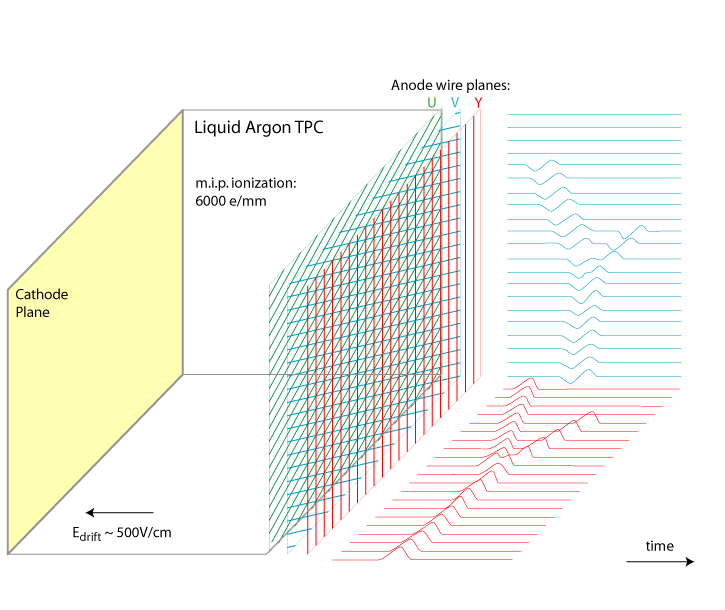
\includegraphics[width=\textwidth,trim=13cm 0cm 0cm 0cm,clip]{signal-15.png}

        %\scriptsize \SI{0.5}{\micro\second} waveform digitization.
      \end{center}
    \end{column}
  \end{columns}

  \vspace{-5mm}

  \footnotesize
  Two general DAQ readout strategies:
  \begin{description}
  \item[Full Stream:] read out entire waveform (\textbf{MicroBooNE})
    \begin{itemize}
    \item \textbf{30GB/s in 120 MB ``events''}.
    \item DUNE at FS would produce 5 TB/s in 25 GB ``events''!
    \end{itemize}
  \item[Zero Supression:] only save waveform parts with significant activity (\textbf{DUNE})
    \begin{itemize}
    \item Threshold chosen based on noise ($E_{thesh} \sim$\SI{0.1}{\mega\electronvolt}/wire)
    \item 2.5 MB/event $\rightarrow$ \textbf{100's TB/year}
    \item requires rejection of natural $^{39}$Ar decay @ \textbf{50 PB/year}
    \end{itemize}
  \end{description}

\end{frame}

